\documentclass{article}
\begin{document}
PhD student Livio Ferrante
Effective Programming Practices - A short report on my hypothetical final project

|
I've created a private repository on Github in my educational account. The URL is https://github.com/livioferrante/my-final-project .
||
In my repository, I've cloned the template that you provided the last day of the course. I'll hypothetically use Python, otherwise I should switch on the branch to specify the language that I'll use most (e.g. stata, r...).
As I showed to you, Waf doesn't run in my machine, then I'm using my repository to put this file about what I would do... if Waf runs!! Therefore, I created a new branch called "report" and I'm working in it  ( git branch report   /   git checkout report ) with a tex file.
|
The ratio behind the use of Waf lies in the reproducibility. Waf is a tool, written in Python, that allows to automate the dependency tracking via a DAG structure (directed acyclic graphs). The replicability of results is an important issue in scientific research and is became a fundamental tool in many economic journals that are implementing strict replication policies. Moreover, it allows to avoid huge waste of time and resources and potential errors.
One could do all it manually by typing stuff to the console and clicking buttons. But it would be hard to track the sequence of clicks and runs one had to do to end up with the final document. So Waf is basically a long list of commands that runs everything in the right order to end up with the final document, presentation and several other things. To make it a little more convenient for the user, Waf can check different folders for the commands, so one doesn't need a huge wscript but can have several small ones located where they'd logically belong.
Currently, I haven't a personal project, then I imagined to implement a simple research which could lead to a creation of an empirical paper.

\begin{figure}[htbp] 
	\centering 
	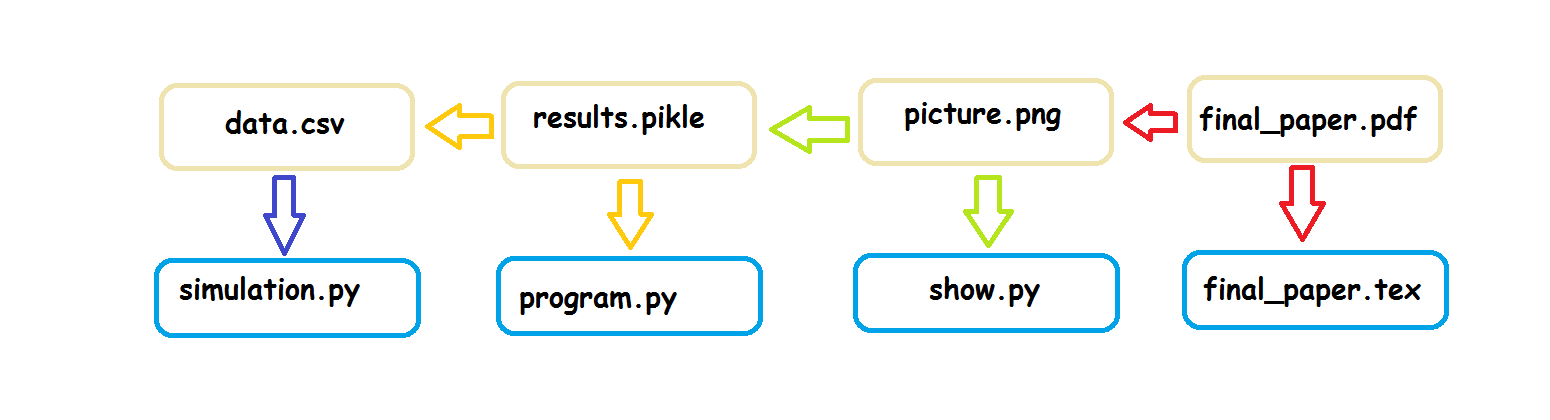
\includegraphics[scale=0.4]
	{effective.png} 
	\caption{Dependency graph} 
	\label{fig:figuraSingola} 
\end{figure}

The colors of arrows distinguish the steps of the analysis: blue is used for data management, orange for the simulation, green for the visualization of a graph, red to get work in a pdf file.
Blue circled nodes represent source files; brown circled nodes represent target files generated by the code depending on source files. 
In the first run, Waf generates all the targets, whereas in the later runs Waf generates only targets for which dependencies are changed. Then Waf is very useful to gain time whenever one runs big projects. 

Wscript files are the entry point for the instructions given to Waf. Every wscript holds build information, that are commands that run the data processing scripts,  computing scripts, plotting scripts, etc. 
Waf works recursively: it means a wscript file checks whether there are any subfolders that also contain wscripts (this is done until the "bottom of the barrel"). By specifying dependencies and targets correctly, wscripts realize what parts depend on each other and whether things could be run in parallel or have to wait for another script to be finished.
First of all, one should set up a suitable folder structure in the source. Folder src (source) contains the structure; all stuff that is created lands in the build folder (bld). 
One has to put the command line to start the process:  
python waf.py configure  

in the main wscript file in order to configure the correct paths:

and inside the file src/wscript:

Now, in order to establish the dependency structure, one has to compile the contents of wscript files.
For the first dependency of the project, one has to put inside the file:


the code:

and so on for the other wscript files, paying attention to the different relationship.

After the configuration, putting the command
python waf.py build
all the wscripts build everything up, and

python waf.py install
some stuff moves in the right place, so it's more available to the user.


Moreover, command clean and distclean could be useful to enforce to rebuild the project. 

This structure is very useful and possibly inevitable for large projects, but comes with some overhead for smaller projects. Also it has some learning curve particularly for non-programmers. Plus it contains many components. all of which have to run otherwise it does not work. 
So, it might be a right way for smaller research projects to make use only of the git part to keep track of different versions and to collaborate. 

Thank you
Livio Ferrante

\end{document}